\chapter{Quick Start Notes}\label{Chap:Quick}
In this chapter, a brief guidance is discussed, which records a quick and easy start for working with NAO. The purpose is that the future students are able to set up the whole environment in their personal PCs and debug everything on it with the help of this note, rather than only using the given Laptop provided by the Lab. The fundamental problems in calibration procedure are also discussed here to give useful suggestions, so that the future student can avoid the problems we met and spent a long time on. The version of code release is from B-Human RoboSoccer team in \cite{BHumanCodeRelease2015}.

\clearpage
\section{Building the project}
After downloading the \textit{BHumanCodeRelease-master.zip} from the git-repository of B-Human team, some more packages are required before building the whole project. For Ubuntu user, the first step can be done by implementing the command as:
\begin{lstlisting}
sudo apt-get install qt4-dev-tools libglew-dew libxm12-dev clang graphviz
\end{lstlisting}
In addition, 32 bit version of \textit{Naoqi} should be downloaded (more details can be found in \cite{robotumwiki}), and be installed with the command:
\begin{lstlisting}
cd <BHuman-CodeRelease>/Install
./installAlcommon.sh <pathto32bitC++NAOQi.zip>
\end{lstlisting}
Then the whole project can be built with:
\begin{lstlisting}
cd <BHuman-CodeRelease>/Make/Linux
make all
\end{lstlisting}

\section{Flashing the robots}
The step-by-step instruction can be found in \cite{BHumanCodeRelease2013}(cf. 2.4). Here are some key-steps:
\begin{enumerate}
    \item Use a USB with the required tools describe in \cite{BHumanCodeRelease2013}.`openNAO-atom-system-image-2.1.4.13.opn' should be downloaded from the "Aldebaran"-website.
    \item Connect the robot with network cable.
    \item Plug in the USB drive into backside of the NAO and press the chest button for a few seconds until the chest flashes blue. The installation will start and the process will be monitored with the help of the LED lights around the robot's ears.
    \item Press the chest button and write down the robot's IP-address, which is important for the further work.
\end{enumerate}

\section{Calibration}
Calibration is very important for the robot. Each time before the game, the calibration should be implemented according to the field and the luminance environment. The calibration process can be done in the application \textit{SimRobot}. A step-by-step guidance in \cite{BHumanCodeRelease2015}(cf. 2.8) can be referred.
\subsection{Joint Calibration}
In order to ensure a stable performance of NAO, joint calibration should be finished first. During the semester, we adjust the joint calibration using the \textit{JointCalibrator}. One thing to mention is that the changes of the calibration is only stored in \textit{BHuman-CodeRelease/Config/Robots/Default} as \textit{jointCalibration.cfg} with the command
\begin{lstlisting}
save representation: JointCalibration
\end{lstlisting}
in \textit{SimRobot}. To save it on NAO, the \textit{copyfile} command should be implemented as:
\begin{lstlisting}
cd <BHuman-CodeRelease/Make/Linux>
./copyfiles <Develop/Debug/Release> <IP_AAA.BBB.CCC.DDD>
\end{lstlisting}
\subsection{Camera and Color Calibration}
There are three modes in Camera Calibration, namely automatic, default and manual. The automatic mode will finish the calibration automatically, but with large deviation to the groundtruth. So the default and manual Calibration are preferred. They can be implemented in the console in SimRobot by
\begin{lstlisting}
call CameraCalibrators/Default
\end{lstlisting}
The default calibration will calculate the result for the upper and lower camera according to the point chosen by us. What important for the point collection is that the point should be collected both in upper camera and in lower camera, so that it will converge faster and easier. \\
If the Default Calibration is not satisfying, the manual calibration can be used with
\begin{lstlisting}
call CameraCalibrators/Manual
\end{lstlisting}
to finely tune the parameter. \fref{CaCl} shows an example of the camera Calibration.
\begin{figure}[!htb]
    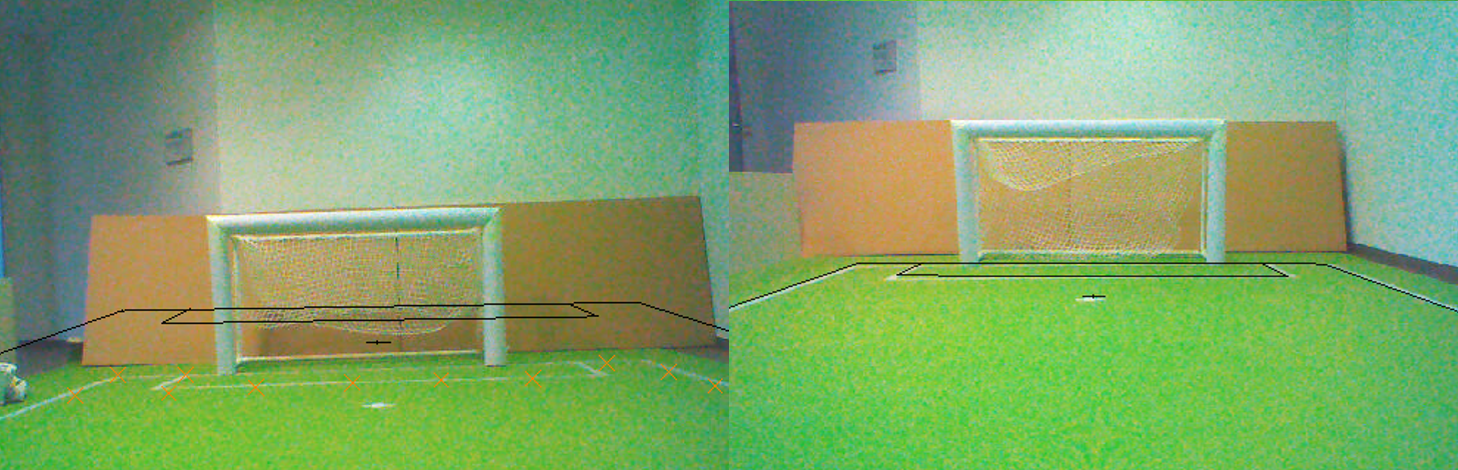
\includegraphics[width=\textwidth]{pics/Camera_Calibration}
    \centering
    \caption{Calibration: Before vs After}
    \label{CaCl}
\end{figure}\\
Color calibration is not as complicated as Joint and Camera Calibration. The only thing to take care is that the color of the ball is \textcolor{orange}{\textbf{orange}}, rather than red.

\section{Coding and Compiling}
\subsection{Tools for coding}
To read and understand the framework of B-Human team in a easier and better way, \textit{CodeLite} proves to be a great tool. B-Human provided a script to automatically generate the workspace for it., which can be found in \textit{Make/LinuxCodeLite/generate}. After installing the \textit{CodeLite}, the whole workspace can be opened like \fref{CoLiIn}.
\begin{figure}[!htb]
    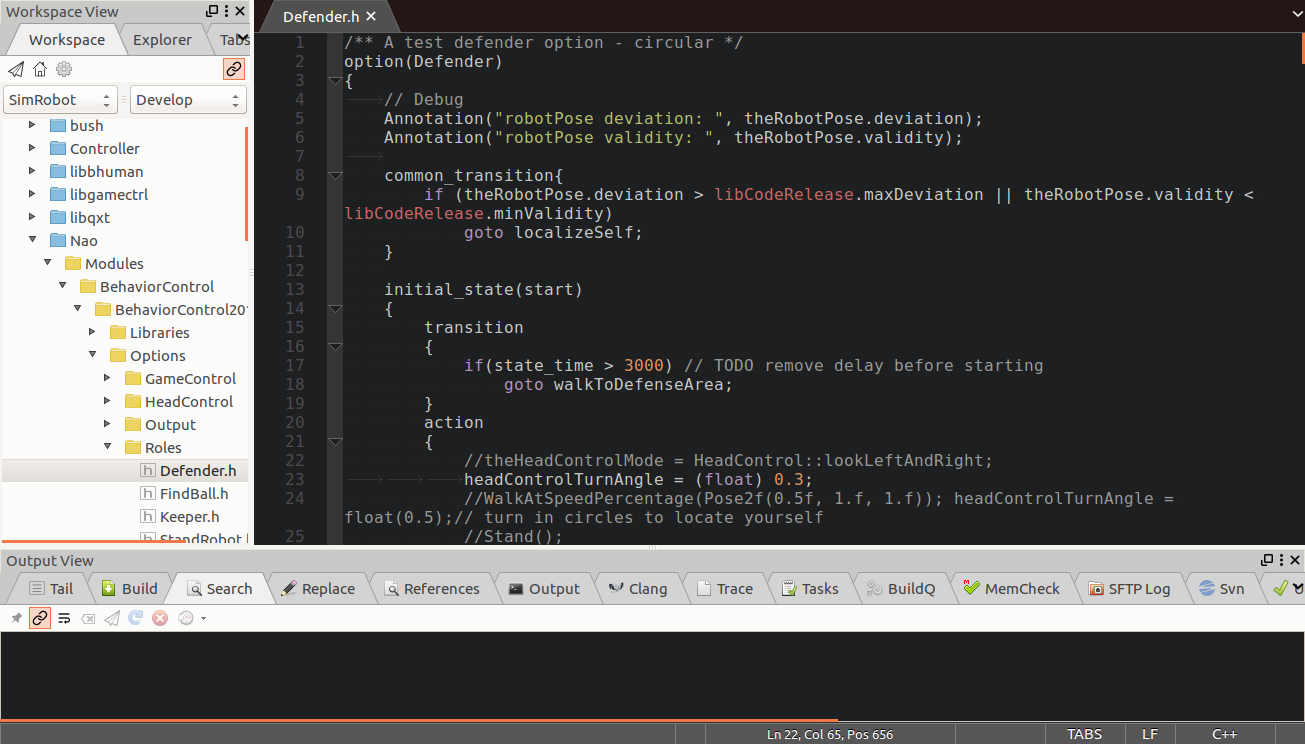
\includegraphics[width=\textwidth]{pics/CodeLite-Interface}
    \centering
    \caption{CodeLite-Interface}
    \label{CoLiIn}
\end{figure}\\
Different variables from different classes defined in various folders can be searched easily with the function ``search in workspace'' in \textit{CodeLite}, which helps the understanding process from beginning.

\subsection{Compiling and Testing in SimRobot}
It is always exciting to test some new ideas immediately on the real robot. But before doing that, implementing the modified code by simulation can be of great help as in SimRobot everything is assumed to behave itself perfectly, such as the camera calibration and joint calibration of the robot. So it should at least behave as one wishes in the SimRobot, then the code can be moved onto the NAO to see the real effects.
To test the modified function in simulation, the application \textit{SimRobot} should be recompiled. From the experience of trial and error, the following command can be executed:
\begin{lstlisting}
cd <BHuman-CodeRelease>/Make/Linux
make all
\end{lstlisting}
As the project is already compiled before, this command will only compile the files which has been changed. So everything related will be compiled without too much consideration.
To see the result in Simulation, run the following command:
\begin{lstlisting}
cd <BHuman-CodeRelease/Build/Linux/SimRobot/Develop>
./SimRobot
\end{lstlisting}
The result can be shown by opening ``Game2015Fast.ros'' located in \textit{BHuman-CodeRelease/Config/Scenes} with the application \textit{SimRobot}.

\subsection{Compiling and Testing on NAO}
To change the code stored in NAO, the function ``copyfiles'' must be used. More concretely, the source file and configuration will then be copied into the `head' of NAO, so that it can perform the new behaviors. Following command can be used:
\begin{lstlisting}
cd <BHuman-CodeRelease/Make/Linux>
./copyfiles <Develop/Debug/Release> <IP_AAA.BBB.CCC.DDD>
\end{lstlisting}
where the first parameter is usually chosen as ``Develop'' and the second parameter is the Network-Address of the NAO you want to program, such as \textit{10.0.29.171}.\\
What to mention here is that the configuration file is also transferred to the NAO. But only the configuration file located in \textit{BHuman-CodeRelease/Config/Robots/Default}. So before \textit{copyfiles}, make sure that the configuration are corresponding to the right one. Our method is to save the configuration file individually and replace it with the corresponding one if the robot changes. 
